\subsection{Structure}

The physical structure of the movement module was designed to be simple, stable, and compatible with the circular "cooking pot" appearance of the final robot. Its geometry allows for efficient assembly and proper distribution of electronic components, motors, and wheels. The chassis consists of two main dodecagonal plates:

\begin{itemize}
    \item A \textbf{lower base plate} that holds the motors, wheels, the battery, and electronics.
    \item An \textbf{upper plate} connected by four vertical rods, providing structural support and space for mounting future upper modules (such as the ticket dispenser).
\end{itemize}

Between the two plates, there's ample vertical space to safely house the internal wiring and maintain separation between moving and static parts. The structural elements were dimensioned using CAD software and detailed in the following technical drawings.

\begin{figure}[H]
    \centering
    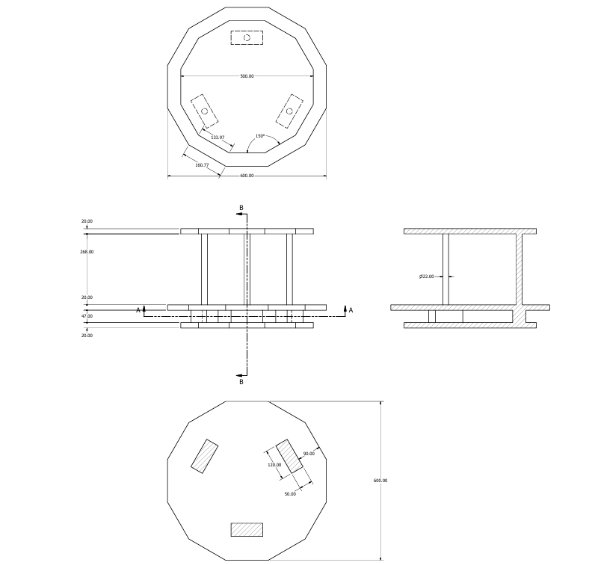
\includegraphics[width=0.8\linewidth]{../ReportMovementModule/images/Aspose.Words.728084da-df58-4b9d-a372-f65cffbdb23d.008.jpeg}
    \caption{Structure Technical Drawings}
\end{figure}

The structure is primarily symmetrical, promoting balance and helping the robot move stably in any direction. This design prioritizes modularity, allowing individual parts to be adjusted, replaced, or expanded without affecting the rest of the system.
